\chapter{Statistics}
\label{stat}
For the next four question we use data from Tradeview taken from coinbase going back to 2016 to the present day. After cleaning the data the head is a follows
\begin{verbatim}
			time	open	high	low	close	Volume	range
date_time							
2016-05-23 10:00:00	1463961600	13.91	13.91	13.61	13.61	0.78673	0.30
2016-05-24 10:00:00	1464048000	13.68	13.74	12.00	12.77	2753.23998	1.74
2016-05-25 10:00:00	1464134400	13.00	13.18	11.93	12.61	9697.18313	1.25
2016-05-26 10:00:00	1464220800	12.61	12.95	12.15	12.47	2989.89229	0.80
2016-05-27 10:00:00	1464307200	12.47	12.47	10.25	10.98	19334.80484	2.22
\end{verbatim}

\section{ What is the average daily range.}
Summary statistics for range.

\begin{verbatim}
count    1565.000000
mean       21.331188
std        34.627367
min         0.100000
25%         4.440000
50%        11.080000
75%        24.380000
max       433.570000
\end{verbatim}
The average daily range is 21.331188. Figure \ref{fig:range} shows the range distribution.
\begin{figure}\label{fig:range}
\center
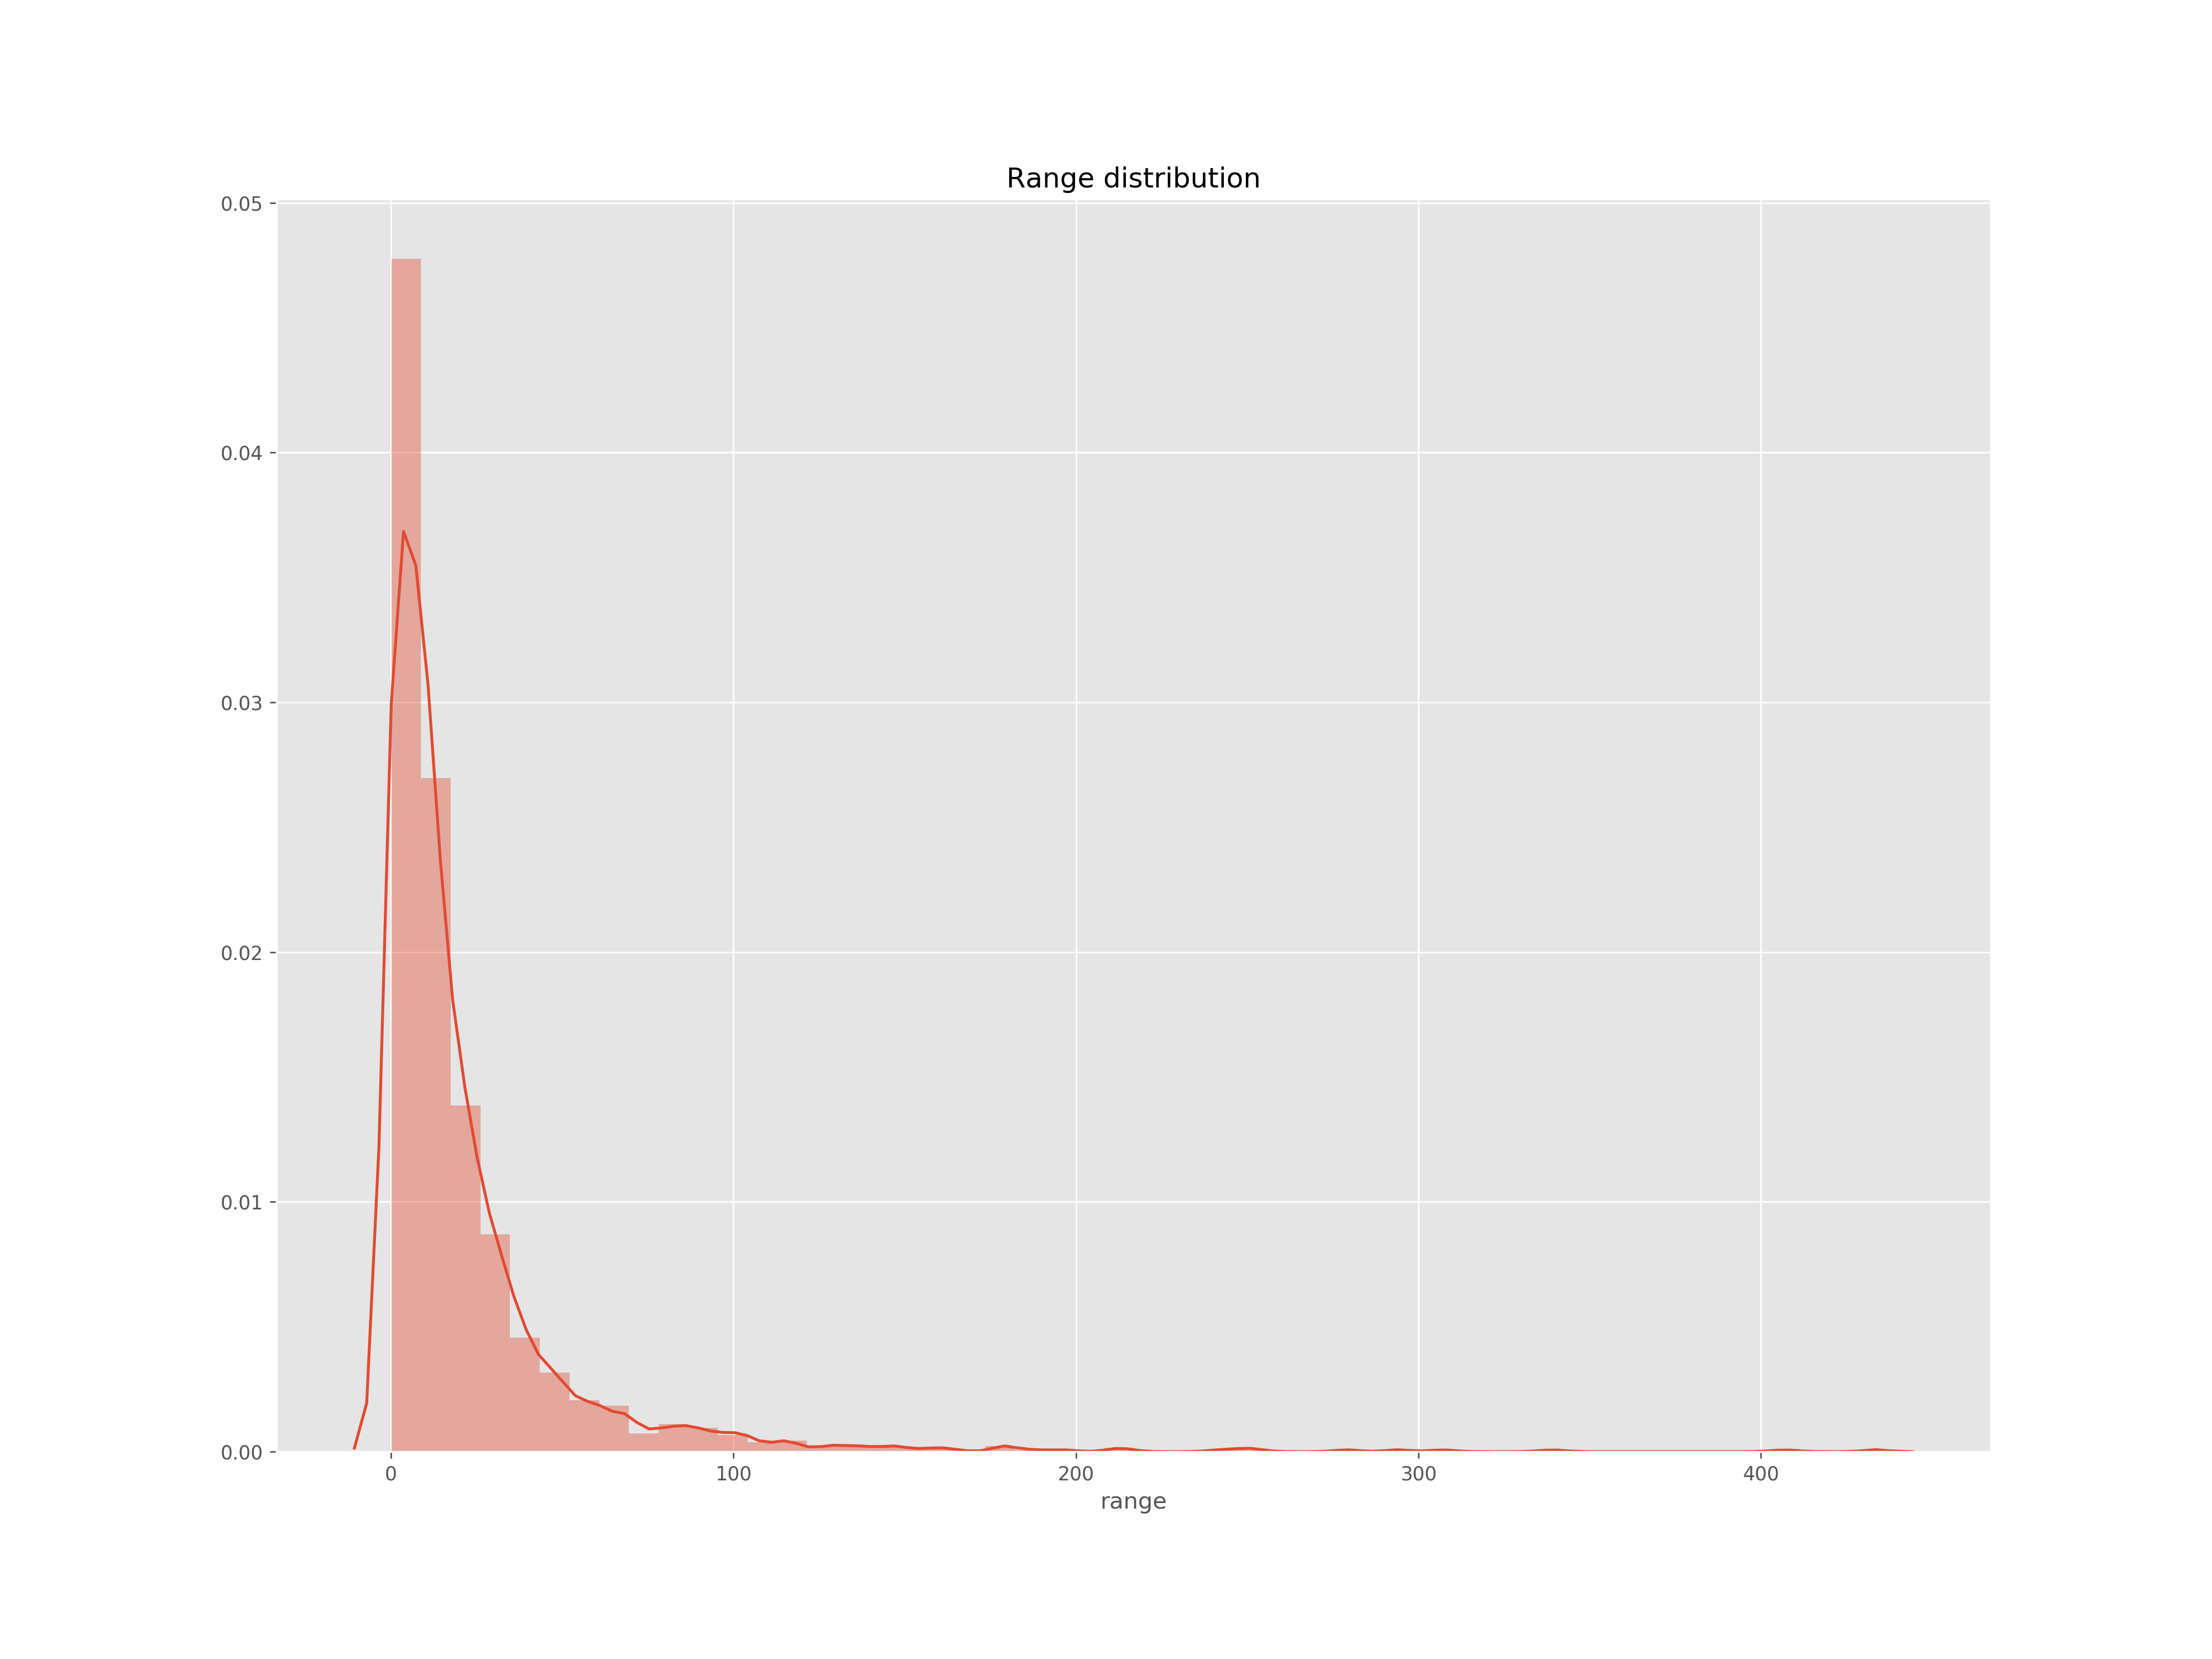
\includegraphics[width=0.9\textwidth]{fig/range.png}
\caption{Range distribution}
\end{figure}

\section{ What is the average daily volume.}
Summary statistics for Volume.

\begin{verbatim}
count    1.565000e+03
mean     1.333461e+05
std      1.276997e+05
min      7.867300e-01
25%      5.343518e+04
50%      9.512464e+04
75%      1.669171e+05
max      1.322283e+06
\end{verbatim}
The average daily Volume is 1.333461e+05. Figure \ref{fig:vol_dist} shows the volume distribution.
\begin{figure}\label{fig:vol_dist}
\center
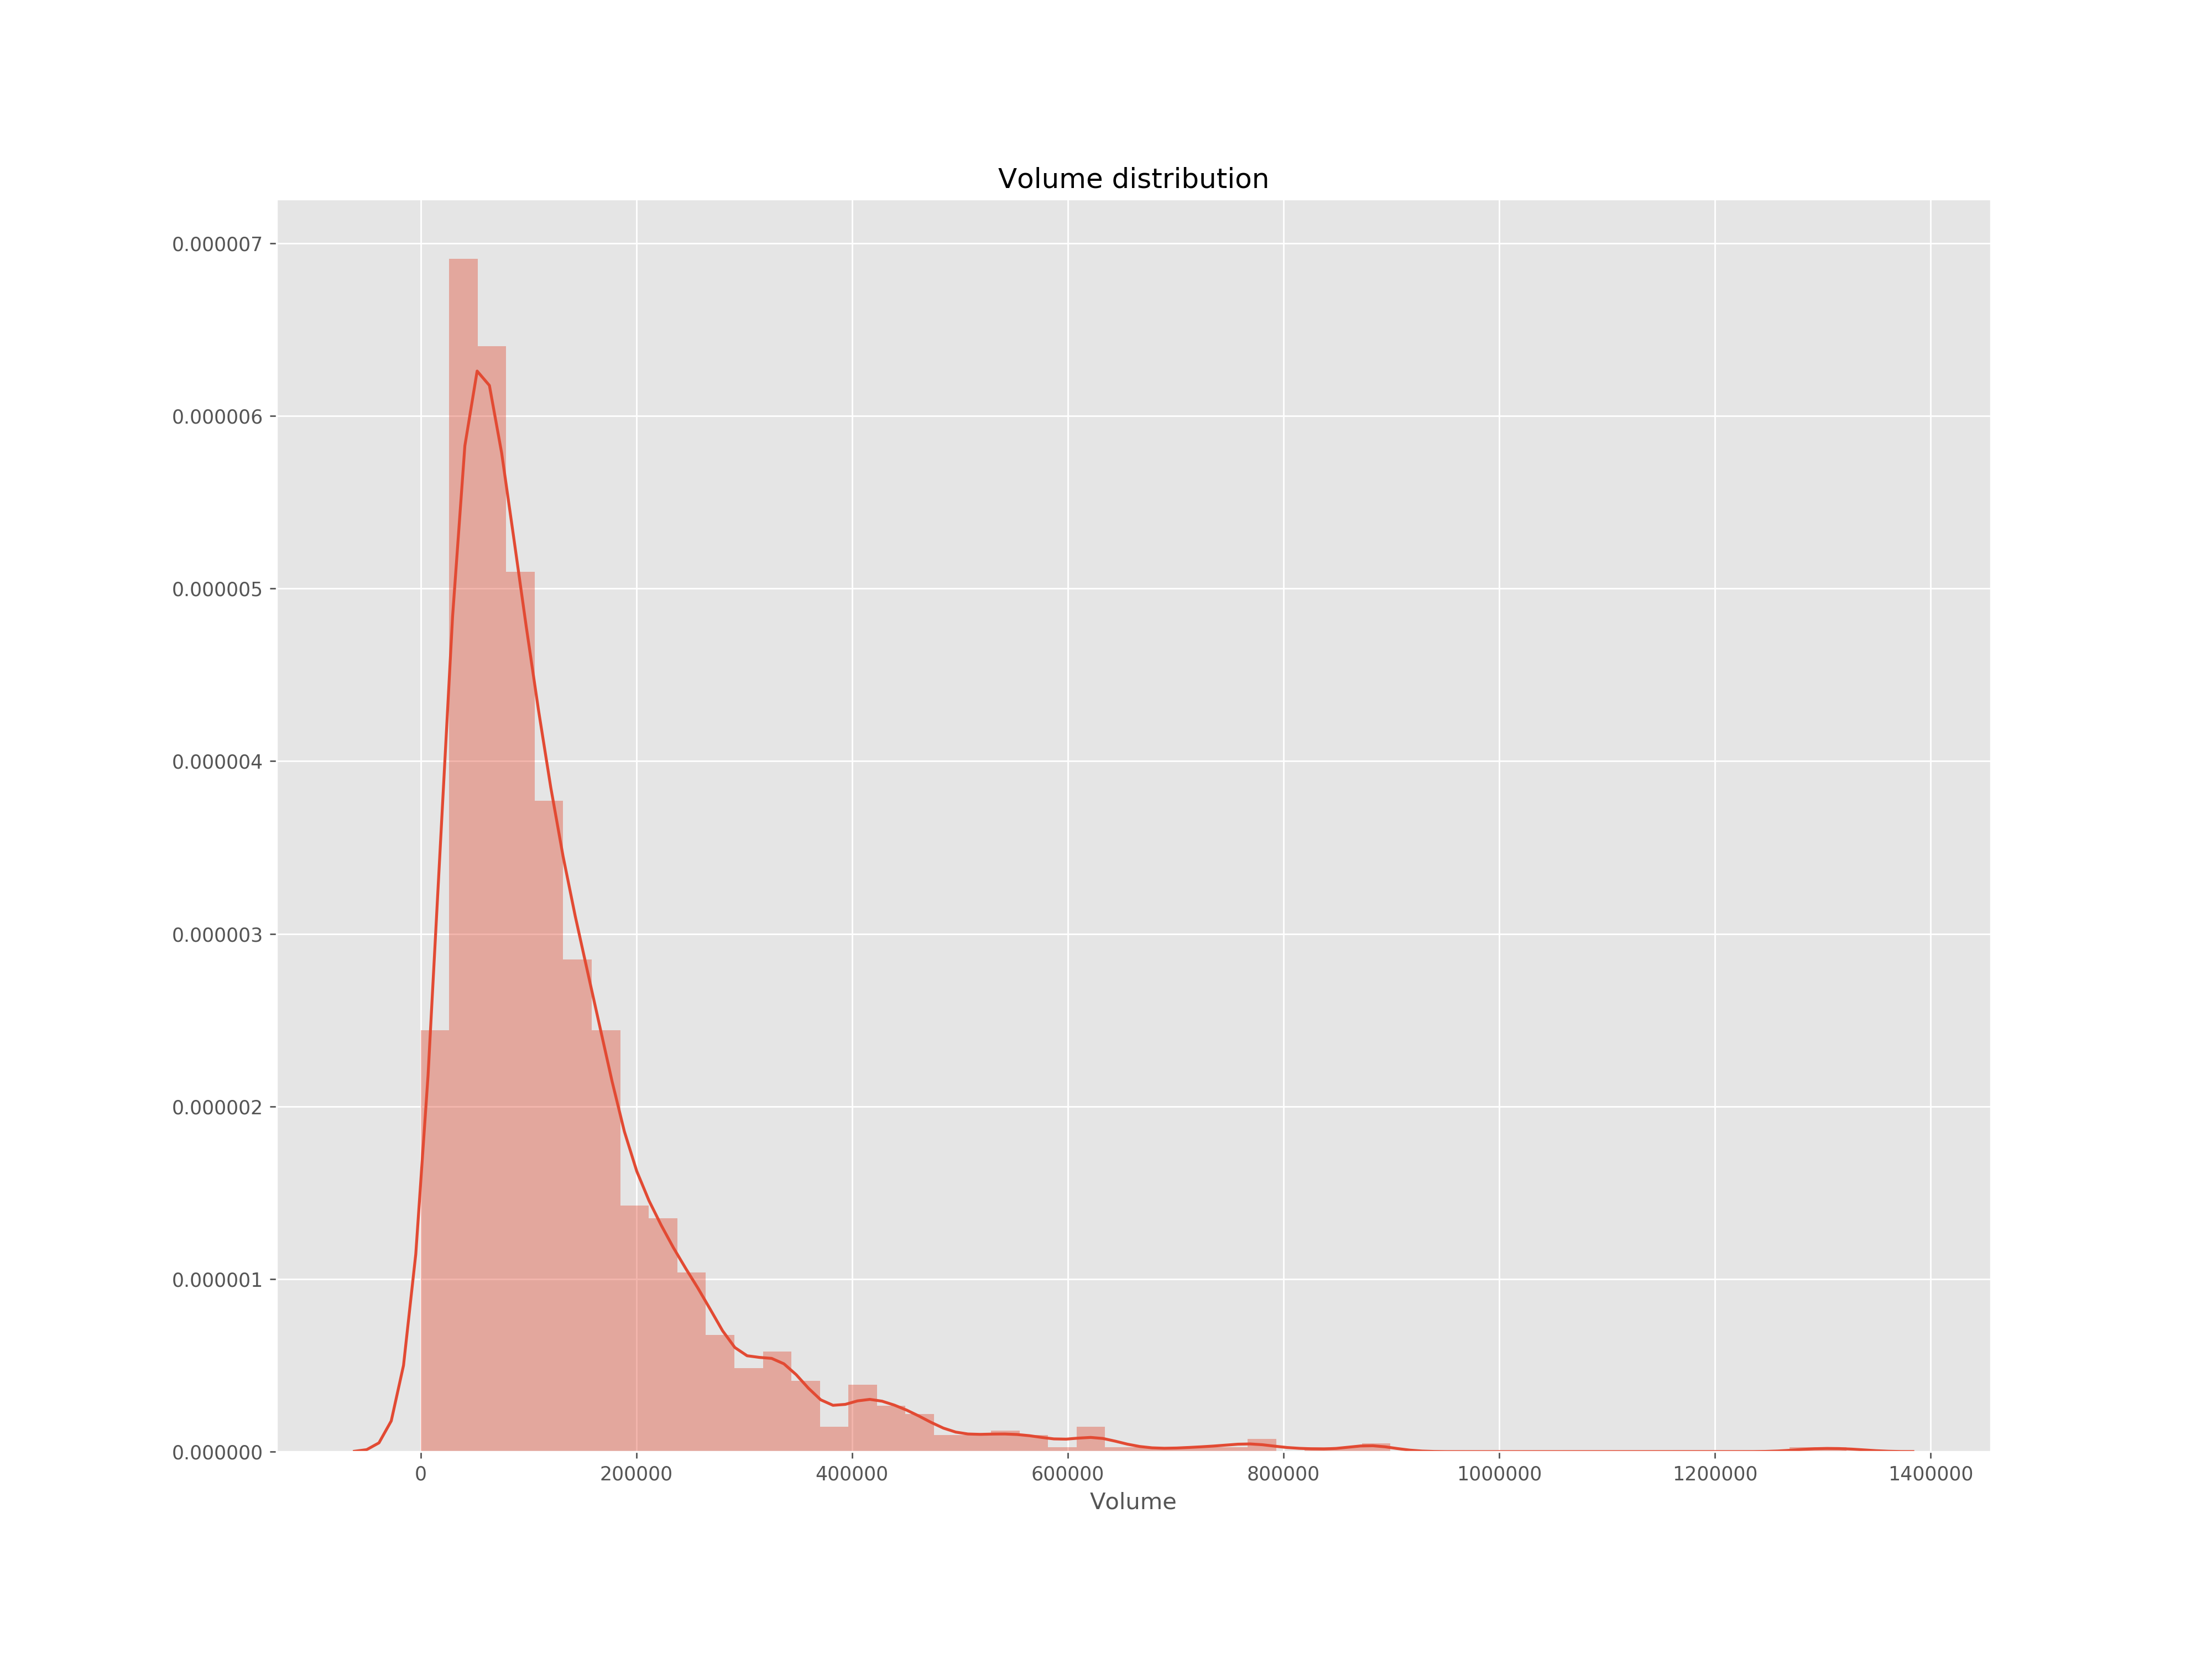
\includegraphics[width=0.9\textwidth]{fig/vol_dist.png}
\caption{Volume distribution}
\end{figure}
\section{ What would you define as a low volume days?}
We will define volume below the 25th percentile to have low volume. Thus, a day with volume below 5.343518e+04 is low.
\section{ What is the average weekend range.}
The data is grouped by day of the week. 0 = Monday,..., 6= Sunday. 

The summary statstics for the groups are

\begin{tabular}{lrrrrrrr}
\toprule
{} &        time &        open &        high &         low &       close &         Volume &      range \\
day &             &             &             &             &             &                &            \\
\midrule
0   &  1531396800 &  244.666652 &  254.059286 &  233.163839 &  244.640179 &  139691.779979 &  20.895446 \\
1   &  1531483200 &  244.642768 &  254.736205 &  231.990179 &  245.165446 &  145372.288791 &  22.746027 \\
2   &  1531569600 &  245.172812 &  255.199821 &  230.065089 &  243.928795 &  150107.028572 &  25.134732 \\
3   &  1531656000 &  243.915134 &  253.779531 &  231.644643 &  242.454085 &  151790.895260 &  22.134888 \\
4   &  1531440000 &  241.549215 &  251.391749 &  229.833072 &  243.245695 &  141879.322847 &  21.558677 \\
5   &  1531526400 &  243.247578 &  253.825830 &  236.150538 &  246.119417 &  100524.152772 &  17.675291 \\
6   &  1531612800 &  246.120852 &  254.312287 &  235.164081 &  245.684126 &  103816.814631 &  19.148206 \\
\bottomrule
\end{tabular}

Thus the average weekend range

$$\frac{17.675291+ 19.148206}{2} = 18.4117485$$

In addition we plot the boxplots of ranges per day give by Figure \ref{fig:rday}. There is no evidence to suggest weekends range more. 
\begin{figure}\label{fig:rday}
\center
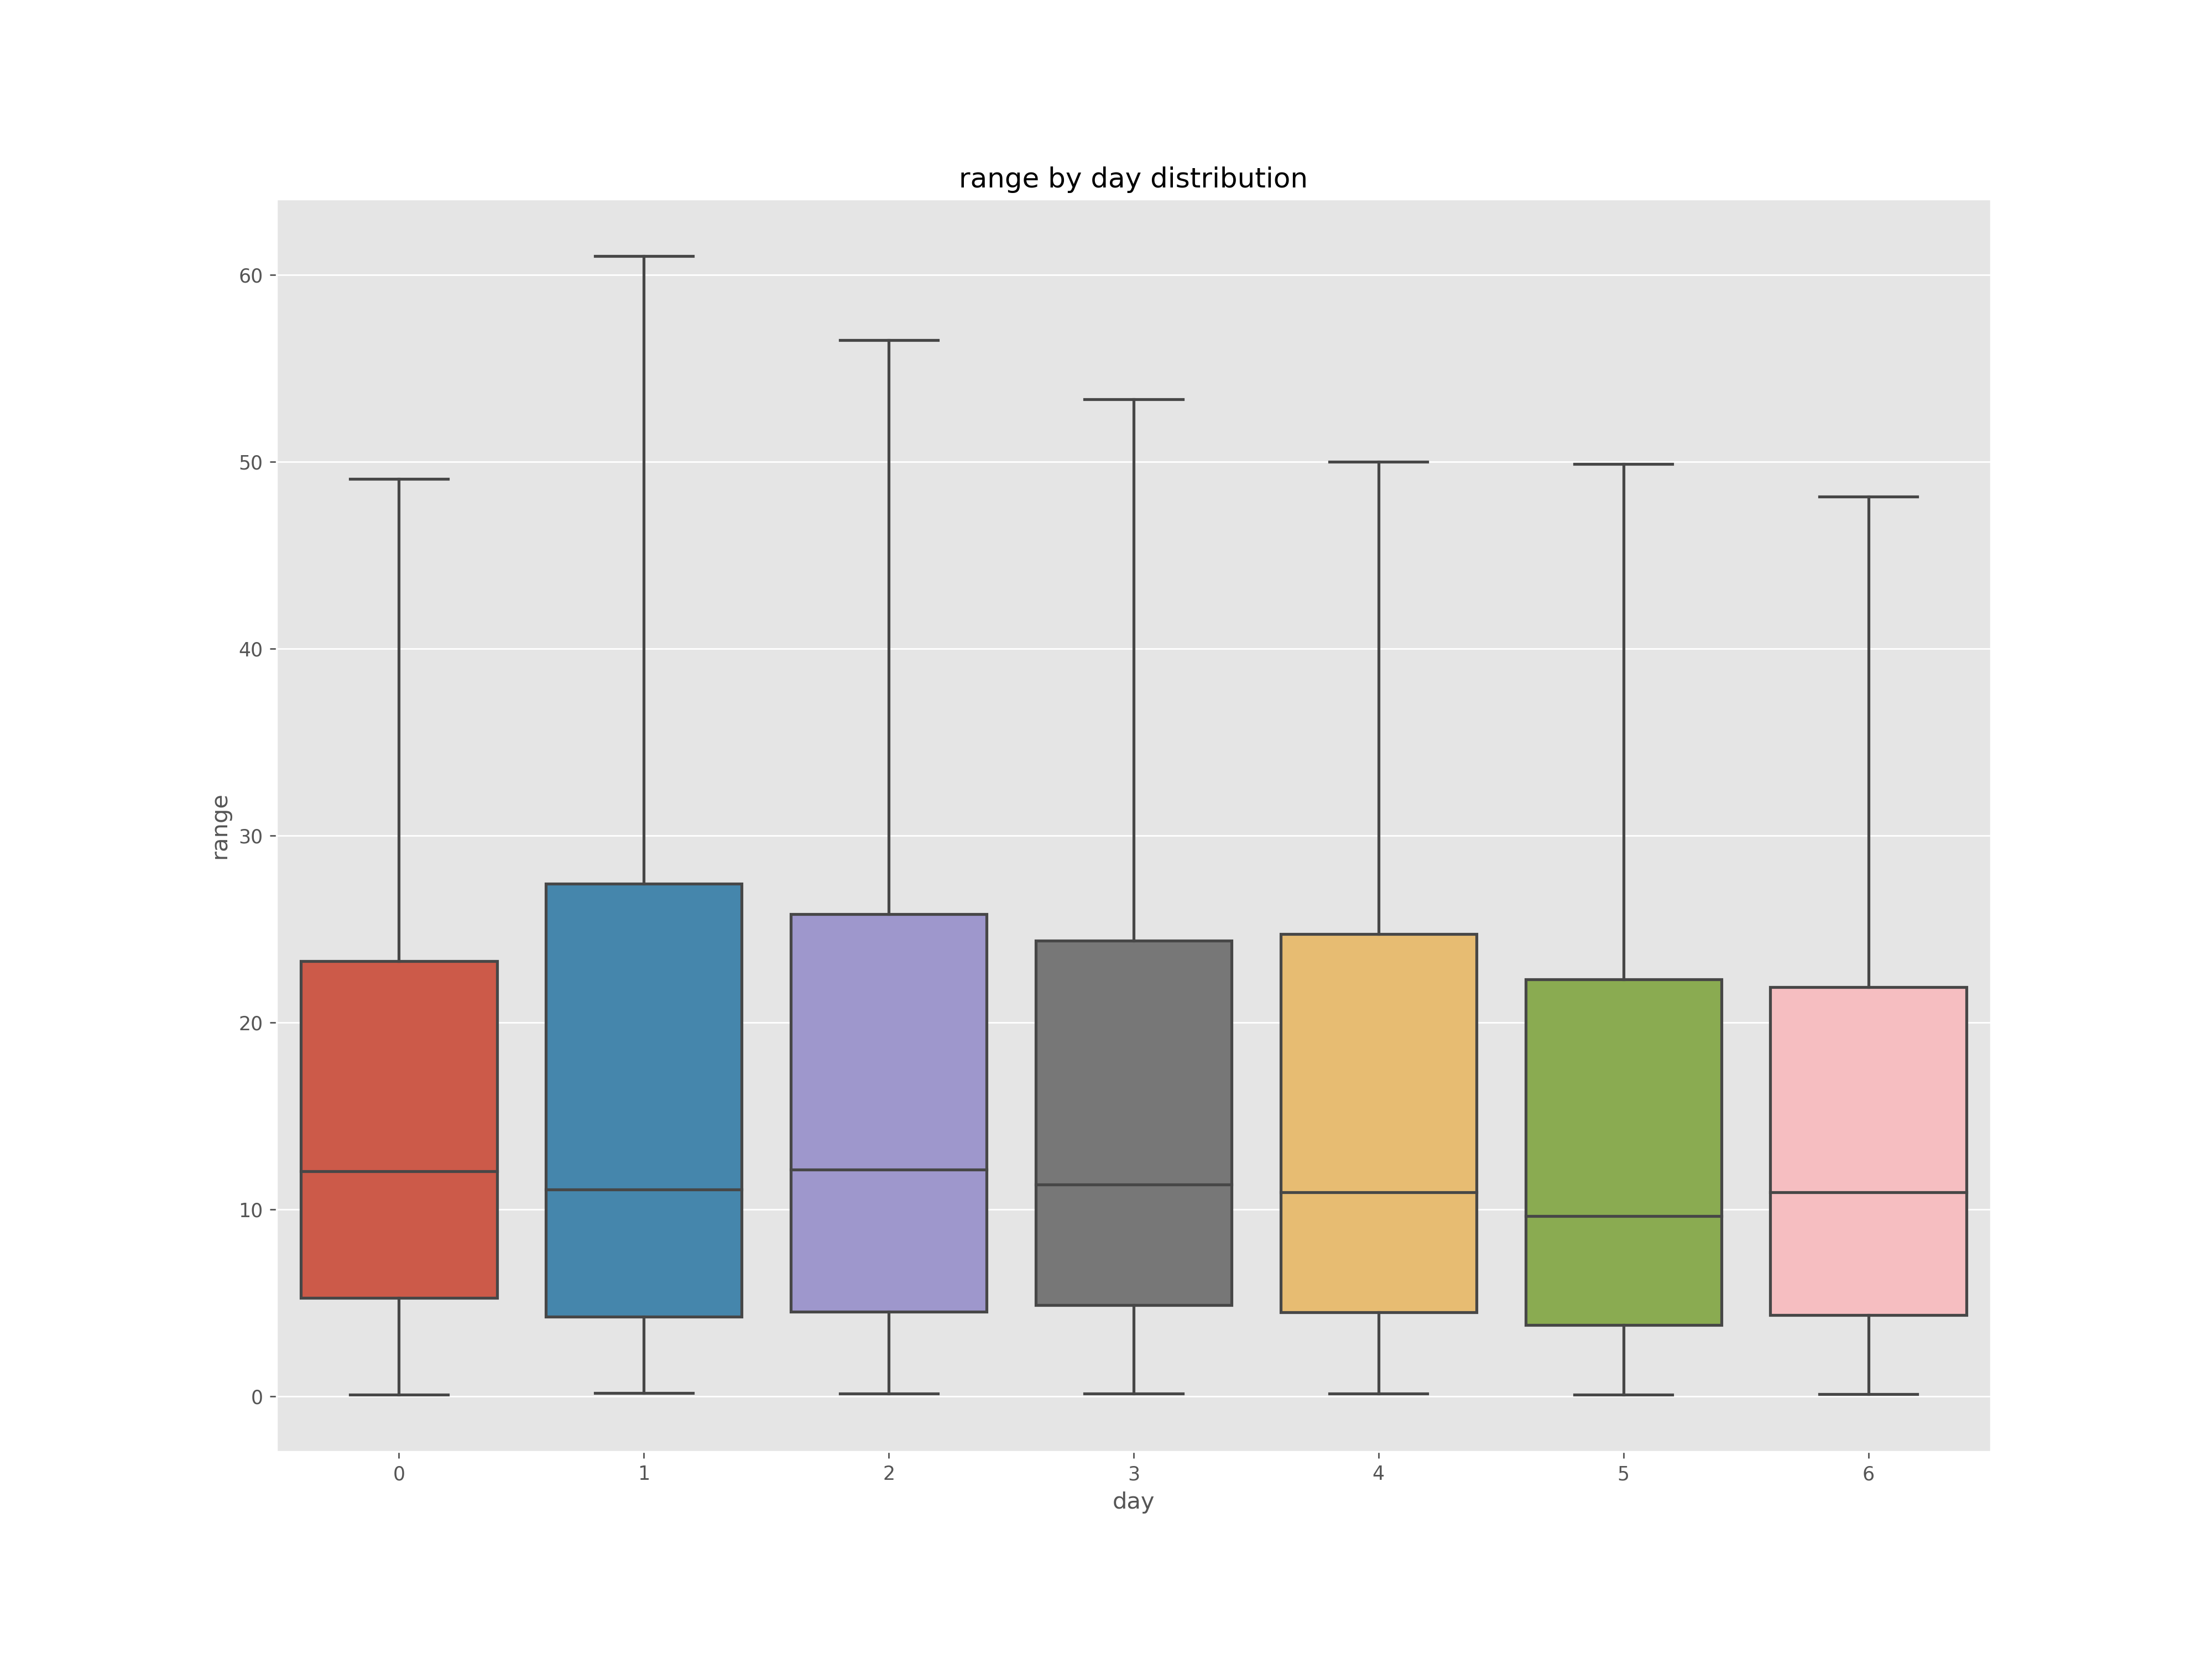
\includegraphics[width=0.9\textwidth]{fig/rday.png}
\caption{Range box plots by day}
\end{figure}
\section{ What affect does an increase in open interest have on price?}
\section{ What affect does a decrease in open interest have on price?}
\section{ Does any relationship exist between open interest and price?}

First we will define the Euro, Asia, USA sessions

\begin{itemize}
\item Euro - WE define this to be when the London stock exchange open

8am to 4 pm UTC or 5pm to 1 am AEST
\item Euro - WE define this to be when the London stock exchange open

8am to 4 pm UTC or 5pm to 1 am AEST
\item USA -
The NYSE/Nasdaq opens at 9:30 a.m. and closes at 4:00 p.m. EST.
EST is GMT minus 5 hours.

Due daylight saving opening and closing times vary slightly. We will just use 12:30am to 7am AEST. This is 2pm to 10pm UTC
\end{itemize}
\section{ What is the average session range and volume - asia euro usa.}
\section{ Work out the ATR of Eth in excel and read the ATR pdf.}
\section{ Work out the distribution of returns and read the pdf.}
\section{ What is the most common time of day for price movements.}
\section{ What are the most common times with the most volume.}
\section{ Is beginning of the month typically quieter then end of month?}
\section{ List of days where it trades greater then its Standard deviation, check (1SD, 2SD, 3SD)}
\section{ Is the market more likely to go up or down?}

\section{ How does the market move when it is $>5  \%  $ move in a day}
\section{ How does the market move when its $>10 \% $ in a day}
\section{ How does it move when its under $<5 \% $?}
\section{ What are the days before and after like of both $>5 \% $ and $<5 \% $ and $> 10 \% $}
\section{ Does it tend to trend or range more?}
fdlgjlskdjgvsdgvdsvsadvfgasdvf
\section{ Do stationary test}
\section{If you used the POC as the fair value for the next trading day, how often does price come back to test this area? (Point of Control)}
\section{Does over average in volume generally relate to bigger price movements? Does this generally last for more then one day?}
\section{Average transactions on the network per day}
\section{Does increase in transactions increase demand and price?}